\chapter{Regulatorische Anforderungen}

\section{Rechtliche Grundlagen}

Auf den ersten Blick können die vielfältigen Regulatorien (Normen, Verordnungen, Richtlinien, Gesetze, \dots) in der Medizintechnik sehr verwirrend sein. Auf den zweiten Blick erkennt man jedoch eine klare, einfache Hierarchie der Regelwerke. Als Ausgangspunkt dient ein ganz einfacher Grundsatz: 
\begin{quote}
	Der Inverkehrbringer eines Medizinproduktes muss die Gesetze all jener Länder einhalten, in welchen er aktiv werden will.
\end{quote}

Daraus ergeben sich bereits drei unabhängige, zentrale Fragestellungen:
\begin{enumerate}
	\item Ist mein Produkt ein Medizinprodukt?
	\item Bin ich für dieses Medizinprodukt der Inverkehrbringer?
	\item Wie kann ich das Gesetz einhalten?
\end{enumerate}

\subsection{Ist mein Produkt ein Medizinprodukt?}

Wann ein Produkt ein Medizinprodukt ist, wird in der Schweiz in der Medizinprodukteverordnung festgehalten. Sinngemässe Definitionen gibt es auch in anderen europäischen Staaten. Ein Produkt muss folgende Kriterien erfüllen, um als Medizinprodukt zu gelten:
\begin{itemize}
	\item Technisches Produkt
	\item Anwendung beim Menschen
	\item Abgrenzung zu Pharmazeutika: diese sind keine Medizinprodukte.
\end{itemize}
Zudem muss es bei einem der vier folgenden Anwendungsfällen benutzt werden:
\begin{itemize}
	\item Erkennen, verhüten, überwachen, behandeln, lindern Krankheiten
	\item Erkennen, überwachen, behandeln, lindern Verletzungen oder Behinderungen
	\item Untersuchen, verändern ersetzen den anatomischen Aufbau oder einen physiologischen Vorgang
	\item Diagnose und Regelung der Empfängnis
\end{itemize}
Dazu einige Beispiele:
\begin{itemize}
	\item Ein \textbf{Heftpflaster} ist ein Medizinprodukt, weil es eine Verletzung lindert.
	\item Ein \textbf{Sturzhelm} ist kein Medizinprodukt, weil er Verletzungen verhütet (Produkte, welche Verletzungen verhüten, gelten als persönliche Schutzausrüstung und fallen damit unter andere Regelungen).
	\item Ein \textbf{Kondom} ist ein Medizinprodukt, weil es sowohl Krankheiten verhütet als auch die Empfängnis regelt.
	\item Eine \textbf{Zahnbürste} verhütet Krankheiten und erfüllt auch alle drei Muss-Kriterien. Trotzdem fallen Zahnbürsten in den meisten Ländern nicht unter die Medizinprodukte, sondern werden als Ausnahme behandelt und als Kosmetika definiert.
	\item Ein \textbf{Aspirin} lindert zwar Krankheiten, entfaltet seine Wirkung jedoch pharmakologisch. Damit ist Aspirin kein Medizinprodukt, sondern ein Pharmazeutikum.
\end{itemize}

\subsection{Bin ich für dieses Medizinprodukt der Inverkehrbringer?}

Die Frage nach dem Inverkehrbringer eines Medizinproduktes ist von wichtiger Bedeutung, weil er für die Erfüllung der gesetzlichen Anforderungen verantwortlich gemacht wird. Zum Inver-kehrbringer wird, wer das Produkt erstmalig einem (potenziellen) Vertreiber oder einem Anwen-der überlässt. In der Regel ist der Hersteller eines Produktes auch der Inverkehrbringer.

\subsection{Wie kann ich das Gesetz einhalten?}

Die Bundesverfassung ermöglicht das Heilmittelgesetz, welches die Anforderungen sowohl für Arzneimittel als auch für Medizinprodukte festlegt. Die Forderungen im HMG sind aber viel zu ungenau für die Hersteller und deshalb wird das Gesetz in Verordnungen detaillierter beschrieben. Zudem kann in der Verordnung auf andere Dokumente (z.B. EU-Richtlinie) verwiesen werden, die dann ebenfalls eingehalten werden muss. Die schweizerische Medizinprodukteverordnung verweist im Wesentlichen auf die europäische Verordnung, in der die Anforderungen noch konkreter beschrieben sind. Diese enge Anbindung der schweizerischen Gesetze an die europäische Medizinprodukterichtlinie erleichtert eine Tätigkeit von Schweizer Medizinprodukteherstellern im europäischen Raum massiv: erfüllt ein Medizinprodukt die Schweizerischen Vorschriften, dann kann dadurch dieses Pro-dukt ohne weitere regulatorische Hürden auch in allen europäischen Ländern in Umlauf gebracht werden.

Normen müssen entgegen der weit verbreiteten Meinung nicht eingehalten werden. Die internationalen Normen können jedoch beigezogen werden, um nachzuweisen, dass einzelne Forderungen der Medizinprodukterichtlinie erfüllt werden und um die Sicherheit eines Produktes nachzuweisen.

Und was passiert, wenn ein Hersteller das Heilmittelgesetz nicht einhält? In Art. 86 des Heilmit-telgesetzes ist festgelegt, dass jemand, der gewerbsmässig handelt und Medizinprodukte, die den Anforderungen des Gesetzes nicht entsprechen, in Verkehr bringt, mit bis zu fünf Jahren Gefängnis und einer Busse von bis zu CHF 500‘000.00 bestraft werden kann.

\section{Anforderungen}

Die europäische Medizinprodukterichtlinie stellt Anforderungen an das eigentliche Medizinprodukt und an die Unternehmensorganisation des Herstellers. Abbildung \ref{fig:ueberwachung-anforderungen} zeigt, wie diese Anforderungen in Europa bzw. den USA überwacht werden.

\begin{figure}
	\centering
	\begin{subfigure}[b]{0.3\textwidth}
		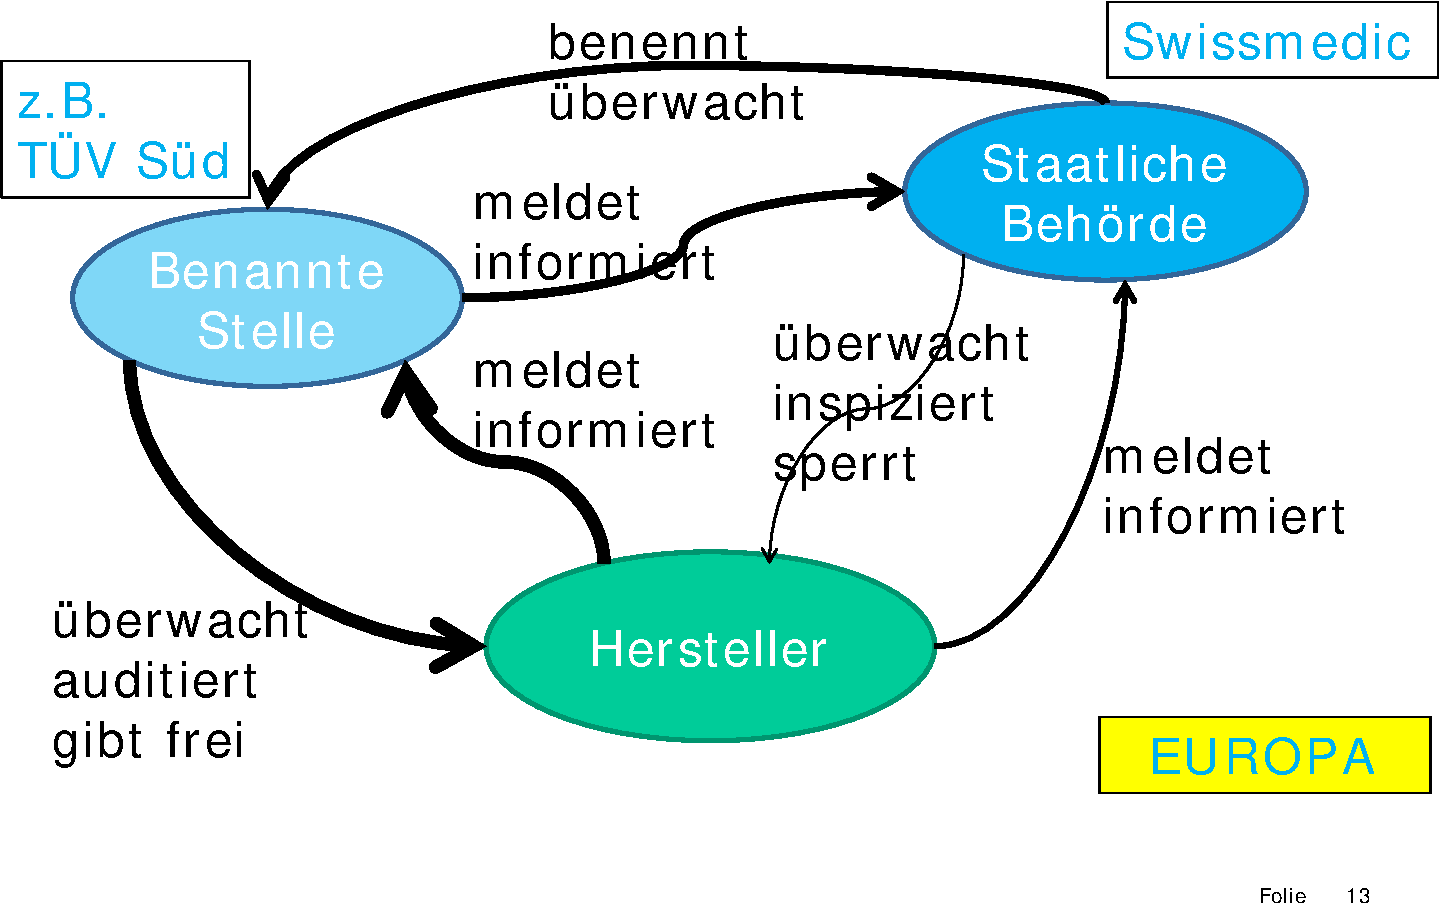
\includegraphics[width=\textwidth]{fig/anforderungen-europa}
		\caption{Europa}
	\end{subfigure}
	~
	\begin{subfigure}[b]{0.3\textwidth}
		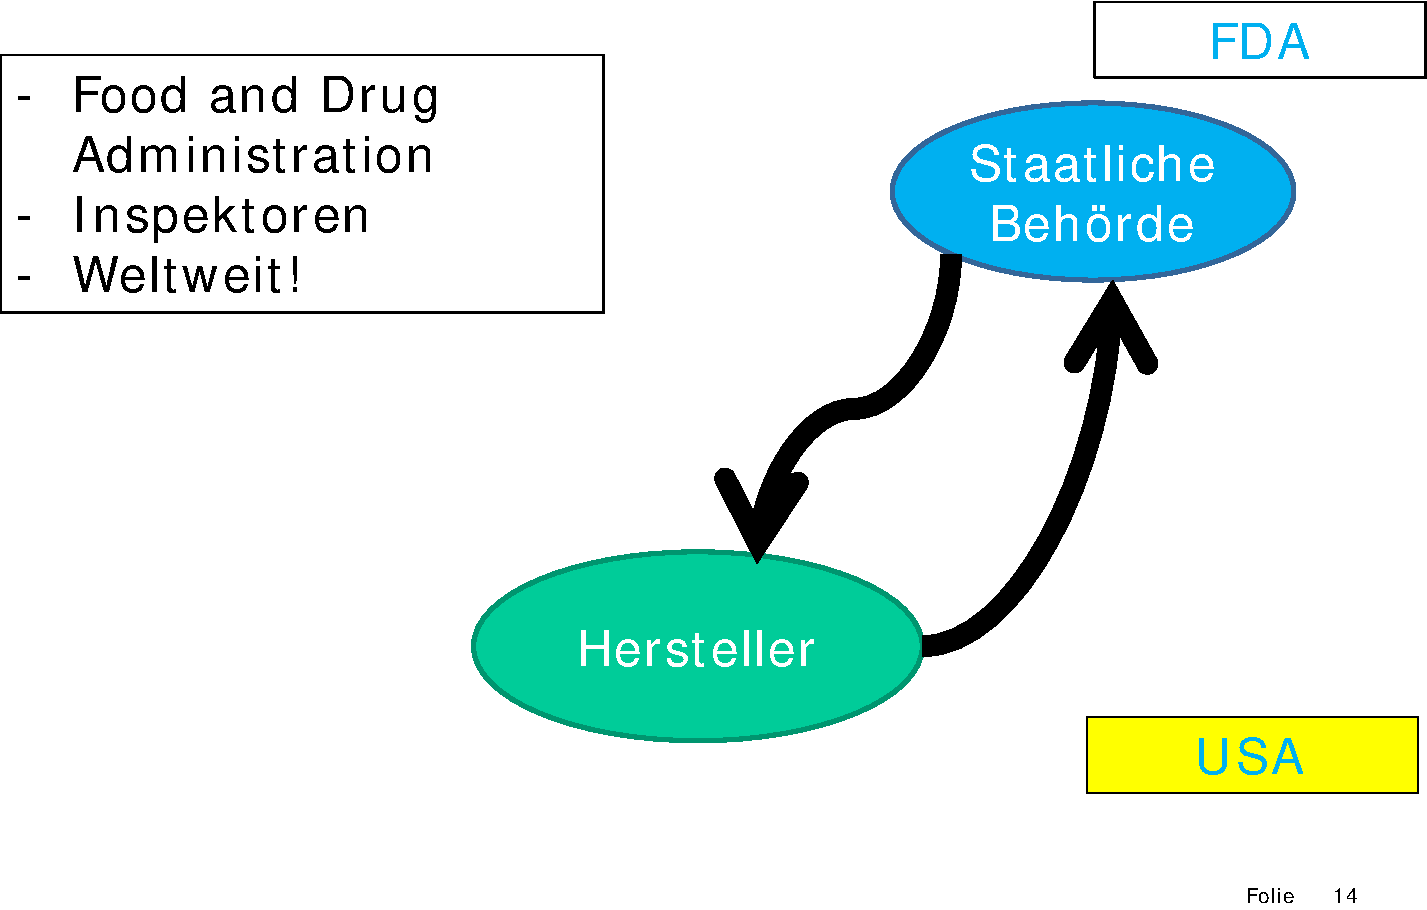
\includegraphics[width=\textwidth]{fig/anforderungen-usa}
		\caption{USA}
	\end{subfigure}
	\caption{Überwachung der Anforderungen}
	\label{fig:ueberwachung-anforderungen}
\end{figure}

Um die Einhaltung der Anforderungen an ein Medizinprodukt nachzuweisen, muss zuerst eine Zweckbestimmung durchgeführt werden. Die Zweckbestimmung beschreibt die Verwendung, für die das Medizinprodukt bestimmt ist. Die Definition der Zweckbestimmung ist Sache des Herstellers.

Da die Anforderungen nicht an alle Medizinprodukte identisch sind, muss nach der Zweckbestimmung eine Klassifizierung der Medizinprodukte vorgenommen werden. Medizinprodukte können in folgende Klassen eingeteilt werden:
\begin{description}
	\item[Klasse I:] Gehhilfen, Rollstühle, wiederverwendbare chirurgische Instrumente
	\item[Klasse IIa:] Einmalspritzen, Hörgeräte, Kontaktlinsen
	\item[Klasse IIb:] Anästhesiegeräte, Blutbeutel, Defibrillatoren, Kondome, Dentalimplantate
	\item[Klasse III:] Künstliches Kniegelenk, Stents, Brustimplantat, Herzschrittmacher
\end{description}
Die Klassifizierung erfolgt entweder direkt mit den in der Medizinproduk-terichtlinie festgelegten Regeln oder mit etwas übersichtlicheren Tabellen, Entscheidungsdia-grammen oder Apps.

Nachdem das Medizinprodukt einer Klasse zugewiesen wurde, muss der Inverkehrbringer eines Medizinproduktes muss nachweisen, dass die grundlegenden Anfor-derungen der Medizinprodukterichtlinie erfüllt wurden. Diese grundlegenden Anforderungen sind im Anhang I der Richtlinie detailliert beschrieben. Wenn ein Hersteller ein neues Produkt in Umlauf bringen will, werden unabhängige Experten («benannte Stelle») überprüfen, ob diese grundlegenden Anforderungen erfüllt sind. Dieser Nachweis kann nur über eine entsprechend umfangreiche schriftliche Dokumentation erfolgen.

\section{Qualitätsmanagementsystem}

Zur dauerhaften Gewährleistung von Sicherheit und die Wirksamkeit eines Medizinproduktes genügt es nicht, dass das Produkt selber die grundlegenden Anforderungen erfüllt, sondern der Inverkehrbringer selber muss gewisse Anforderungen an seine Organisation erfüllen. Diese Anforderungen an die Unternehmensorganisation sind in der Norm ISO 13485 beschrieben. Die ISO 13485 ist in vielen Punkten identisch mit der besser bekannten ISO 9001, legt den Schwerpunkt jedoch auf Produktsicherheit, während die ISO 9001 auf die kontinuierliche Verbesserung ausgelegt ist. Nachfolgend sind die wesentlichen Unterschiede zwischen der ISO 13485 und der ISO 9001 kurz beschrieben:
\begin{description}
	\item[Erfüllung der Kundenanforderungen] \hfil \\
	Ein Medizinprodukt muss die expliziten, impliziten und gesetzlichen Anforderungen seiner Kunden erfüllen. Für fehlerhafte Produkte welche die Anforderungen nicht erfüllen, muss ein Prozess für Korrektur- und Vorbeugemassnahmen vorhanden sein. Zudem muss ein Prozess für Kundenreklamationen und ein Prozess für das Melden von Ereignissen an die Behörden definiert sein.
	
	\item[Managementverantwortung] \hfil \\
	Das Mgmt muss die Verfügbarkeit von Ressourcen insbesondere im QM-Bereich sicherstellen. Das Mgmt muss die Verantwortungen, Befugnisse und Kenntnisse der Mitarbeiter festlegen und dokumentieren. Zudem stellt es sicher dass die beschriebenen Prozesse eingehalten und gelebt werden.
	
	\item[Produktentwicklung] \hfil \\
	Die Produktentwicklung wird in Kapital \ref{sec:produktentwicklung} näher thematisiert.
	
	\item[Validierung von Prozessen zur Produktion und zur Dienstleistungserbringung] \hfil \\
	Eine Validierung ist der Nachweis, dass ein bestimmter Prozessschritt dauernd ein Ergebnis er-zeugt, das die vorgegebenen Anforderungen erfüllt. Dies kann durch Versuche nachgewiesen werden.
	
	\item[Kontrolle der Arbeitsumgebung] \hfil \\
	Hygiene und Sauberkeit spielen bei der Produktion von Medizinprodukten eine zentrale Rolle, da bei ungenügender Beachtung dieser beiden Aspekte die Sterilität und die Bioverträglichkeit be-einträchtigt werden könnten. Deshalb sind sowohl die Hygiene und auch die Sauberkeit in der Produktion detailliert festzulegen.
	
	\item[Risikomanagementprozess] \hfil \\
	Das Risikomanagement wird in Kapital \ref{sec:risikomgmt} näher thematisiert.
	
	\item[Qualifizierung von Lieferanten] \hfil \\
	Wenn ein Hersteller bestimmte Teile seines Medizinproduktes von einem Lieferanten bezieht, ist es in der Verantwortung des Herstellers diesen auch zu Qualifizieren. Deshalb werden z.B. regelmässig Audits beim Lieferanten oder Eingangskontrollen der Waren durchgeführt.
	
	\item[Produktherstellung und Rückverfolgbarkeit] \hfil \\
	Wenn ein Fehler auftritt muss die Rückverfolgung gewährleistet sein und das schon innerhalb der Herstellung. Dies ist hilfreich um einen Fehler zu beheben oder einen Produkterückruf durchzuführen.
\end{description}